\documentclass{standalone}

\usepackage{tikz}
\usetikzlibrary{arrows.meta}


\begin{document}

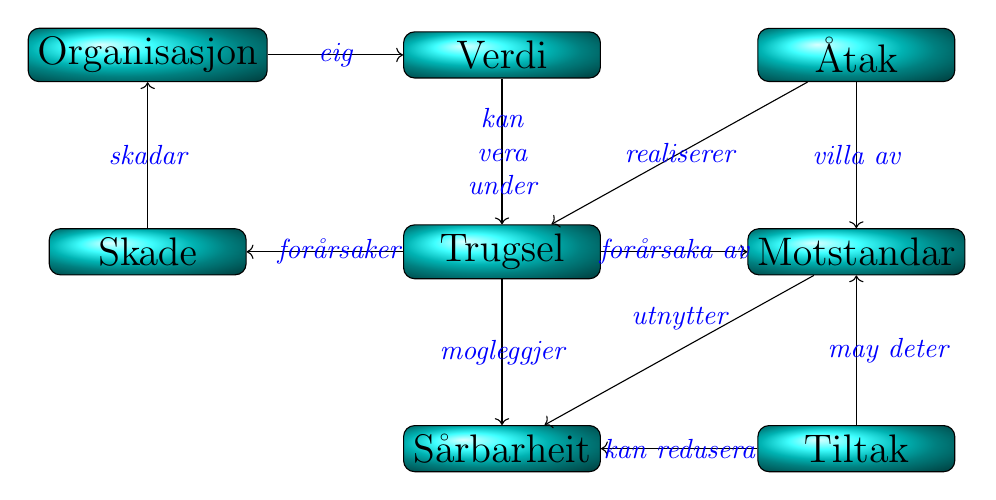
\begin{tikzpicture}
      \tikzstyle{term}=[minimum width=25mm,font=\Large,rounded corners,draw,ball color=cyan]
  \tikzstyle{lab}=[rounded corners,font=\centering\itshape,text=blue]
   \def\pb#1#2{\parbox{#1}{\centering #2}}

  \node [term] (asset) at (4.5,5) {Verdi} ;
  \node [term] (org) at (0,5) {Organisasjon} ;
  \node [term] (threat) at (4.5,2.5) {Trugsel} ;
  \node [term] (impact) at (0,2.5) {Skade} ;
  \path [->,draw] (org) edge node[lab] {\pb{12mm}{eig}} (asset) ;
  \path [->,draw] (asset) edge node[lab] {\pb{12mm}{kan vera under}} (threat) ;
  \path [->,draw] (threat) edge node[lab] {\pb{12mm}{forårsaker}} (impact) ;
  \path [->,draw] (impact) edge node[lab] {\pb{12mm}{skadar}} (org) ;
  
  \node [term] (thsrc) at (9,2.5) {Motstandar} ;
  \path [->,draw] (threat) 
    edge node[lab] {forårsaka av} (thsrc) ;


  \tikzstyle{second}=[ball color=red]
  \tikzstyle{third}=[ball color=yellow]

  \node [term] (vul) at (4.5,0) {Sårbarheit} ;
  \node [term] (control) at (9,0) {Tiltak} ;
  \path [->,draw] (threat) 
    edge node[lab] {\pb{18mm}{mogleggjer}} (vul) ;
  \path [->,draw] (control) edge node[lab] {kan redusera} (vul) ;
  \path [->,draw] (control) edge node[lab,xshift=4mm]
     {\pb{18mm}{may deter}} (thsrc) ;
  \path [->,draw] (thsrc) edge node[lab,yshift=4mm] {utnytter} (vul) ;

  \node [term] (atk) at (9,5) {Åtak} ;
  \path [->,draw] (atk) edge node[lab] {villa av} (thsrc) ;
  \path [->,draw] (atk) edge node[lab] {realiserer} (threat) ;

\end{tikzpicture}
\end{document}
